%!TEX root = draft.tex

\section{Succinct Reference Implementations of Collection Data Types}
\label{sec:succinct reference implementations of collection data types}

$Spec$ is called collection, if

\begin{itemize}
\setlength{\itemsep}{0.5pt}
\item[-] It contains two update methods, one is called $add$ and the other is called $rem$.

\item[-] {\color {red}Given a $add$ operation $o_a \in O$ with $lab(o_a)= add(a)$, let $\mathit{FstRem}(O,\mathit{vis},o_a) = \{ o_r \vert lab(o_r)=rem(a),(o_a,o_r) \in \mathit{vis}$, $ \neg \exists o'_r, lab(o'_r) = rem(a), (o_a,o'_r),(o'_r,o_r) \in \mathit{vis} \}$ be the set of first visible matching remove of $o_a$.

}

%Given a $add$ operation $o_a \in O$ with $lab(o_a)= ADD(a)$, function $f_R(O,\mathit{vis},o_a) = \{ o_r \vert lab(o_r)=$REMOVE$(a),(o_a,o_r) \in \mathit{vis}$, $ \neg \exists o'_r, lab(o'_r) = $REMOVE$(a), (o_a,o'_r),(o'_r,o_r) \in \mathit{vis} \}$ is the set of corresponding REMOVE operations of $o_a$.

\item[-] Let $\mathit{RdtA}(O,\mathit{vis})$ be the set of redundant $add$ operations of $O$: $add$ operation $o_a$ is in $Redt(O,\mathit{vis})$, if for each replica $r$, there exists $o_r \in \mathit{FstRem}(O,\mathit{vis},o_a)$, such that $o_a$ and $o_r$ either happens on or delivered to replica $r$.

\item[-] {\color {red} Given an annotated history $x = (O,\mathit{vis},\mathit{arb})$ and $S \subseteq O$, let $\mathit{frg}(x,S)$ be a annotated history $(O',\mathit{vis}',\mathit{arb})$ obtained from $x$ by forgetting operations in $S$ when $S$ can be forgotten from $O$. $S$ can be forgotten from $O$, if $S$ is a union of $add$ operations $S_a$ and $rem$ operations $S_r$, such that $S_a \subseteq \mathit{RdtA}(O,\mathit{vis})$, and $S_r = \{ o_r \vert  \{ o_a \vert o_r \in \mathit{FstRem}(O,\mathit{vis},o_a) \} \subseteq S_a \}$. By forgetting $S$, we have $O' = O \setminus S$ and $\mathit{vis}' = \mathit{vis} \uparrow_{(O' \times O')}$, and $\mathit{arb}' = \mathit{arb} \uparrow_{(O' \times O')}$. %Here we permit $\mathit{arb}$ to contain more operations than $O$ in annotated history. %, and $\mathit{arb}' = \mathit{arb} \uparrow_{(O' \times O')}$.
}

%\item[-] Predicate $P_{frg}$ is used to check if a set $S$ of operations can be forgotten. Given $S \subseteq O$, $P_{frg}(O,\mathit{vis},S) = \mathit{true}$, if $S = S_a \cup S_r$, such that $S_a \subseteq RdtA(O,\mathit{vis})$, and $S_r = \{ o_r \vert  \{ o_a \vert o_r \in f_R(O,\mathit{vis},o_a) \} \subseteq S_a \}$.

%\item[-] Given an operation context $x = (O,<,\mathit{arb})$ of $o_1$ and $S \subseteq O$, let $forg(x,S)$ be a operation context $(O',<',\mathit{arb}')$ of $o_1$ obtained from $x$ by forgetting operations in $S$: $O' = O \setminus S$, $<' = < \uparrow_{(O' \times O')}$, and $\mathit{arb}'$ is obtained from $\mathit{arb}$ by projection on $O' \cup \{ o_1 \}$.

%\item[-] Given an annotated history $x = (O,\mathit{vis},\mathit{arb})$ and $S \subseteq O$, let $frg(x,S)$ be a annotated history $(O',\mathit{vis}',\mathit{arb}')$ obtained from $x$ by forgetting operations in $S$: $O' = O \setminus S$, $\mathit{vis}' = \mathit{vis} \uparrow_{(O' \times O')}$, and $\mathit{arb}'$ is obtained from $\mathit{arb}$ by projection on $O'$.

%\item[-] An extension of a operation context $(O,<,\mathit{arb})$ of $o_1$ is another operation context $(O',<',\mathit{arb}')$ of $o_1$, such that $O \subseteq O'$, $\mathit{arb}$ is the projection of $\mathit{arb}'$ over $O \cup \{ o_1 \}$ , $< \subseteq <'$, and $<' \cap ( (O'-O) \times O ) = \emptyset$.

\item[-] An extension of an annotated history $(O,\mathit{vis},\mathit{arb})$ is another annotated history $(O',\mathit{vis}',\mathit{arb}')$, such that $O \subseteq O'$, $\mathit{arb}$ is the projection of $\mathit{arb}'$ over $O$ , $\mathit{vis} \uparrow_{(O \times O)} \subseteq \mathit{vis}' \uparrow_{(O' \times O')}$, $\mathit{vis}' \cap ( (O'-O) \times O ) = \emptyset \wedge \mathit{vis}' \cap ( O \times O ) = \mathit{vis}$.

%\item[-] Let $Inv$ be a property that is satisfied by all states which are on executions of $RImp(Spec)$.

%\item[-] Then, we require that, %for operation context that satisfies $Inv$
%    \begin{itemize}
%    \setlength{\itemsep}{0.5pt}
%    \item[-] For each operation context $x = (O,<,\mathit{arb})$ and $S \subseteq O$, where $P_f(O,<,S)$: For each operation $\ell$ and extension $x_1$ of $x$, $x_1 \in Spec(\ell)$, if and only if $forg(x_1,S) \in Spec(\ell)$.

%    \item[-] If $f_R(O,<,S) \wedge forg((O,<,\mathit{arb}),S) = (O',<',\mathit{arb}') \wedge f_R(O',<',S') \wedge forg((O',<',\mathit{arb}'),S') = (O'',<'',\mathit{arb}'')$, then $f_R(O,<,S \cup S')$.
%    \end{itemize}

{\color {red}
\item[-] Then, we require that,
    \begin{itemize}
    \setlength{\itemsep}{0.5pt}
    \item[-] For each annotated history $x = (O,\mathit{vis},\mathit{arb})$ and $S \subseteq O$, where $S$ can be forgotten from $O$: For each operation label $\ell$ and extension $x'$ of $x$, let $y'$ be the operation context of $x'$ and $o \in O$, and let $y''$ be the operation context of $frg(x',S)$ and $o$, then $y' \in Spec(\ell)$, if and only if $y'' \in Spec(\ell)$.

    %$x_1 \in Spec(\ell)$, if and only if $forg(x_1,S) \in Spec(\ell)$.

    %\item[-] If $P_{frg}(O,\mathit{vis},S) \wedge forg((O,\mathit{vis},\mathit{arb}),S) = (O',\mathit{vis}',\mathit{arb}') \wedge P_{frg}(O',\mathit{vis}',S') \wedge forg((O',\mathit{vis}',\mathit{arb}'),S') = (O'',\mathit{vis}'',\mathit{arb}'')$, then $P_{frg}(O,\mathit{vis},S \cup S')$.
    \item[-] If $\mathit{frg}((O,\mathit{vis},\mathit{arb}),S) = (O',\mathit{vis}',\mathit{arb}') \wedge \mathit{frg}((O',\mathit{vis}',\mathit{arb}'),S') = (O'',\mathit{vis}'',\mathit{arb}'')$, then $\mathit{frg}((O,\mathit{vis},\mathit{arb},S \cup S') = (O'',\mathit{vis}'',\mathit{arb}'')$.
    \end{itemize}
}
\end{itemize}


Similarly, we can forget operations $S$ from a state $(O,\mathit{ro},\mathit{del},\mathit{vis})$ by deleting $S$ from $O$, $\mathit{ro}$ and $\mathit{del}$. Given a state $q = (O,\mathit{ro},\mathit{del},\mathit{vis})$, its succinct version $suct(q)$ is obtained from $q$ by forgetting $\mathit{RdtA}(O,\mathit{vis}) \cup \{ o_r \vert  \{ o_a \vert o_r \in f_R(O,\mathit{vis},o_a) \} \subseteq \mathit{RdtA}(O,\mathit{vis}) \}$. Given a collection specification $Spec$, its succinct reference implementation is given as an LTS $SRImp(Spec) = (Q_s,\Sigma,\rightarrow_s,q_0)$, which can be obtained from $RImp(Spec) = (Q,\Sigma,\rightarrow,q_0)$ as follows:

\begin{itemize}
\setlength{\itemsep}{0.5pt}
\item[-] $Q_s$ is the set of $(O,\mathit{ro},\mathit{del},\mathit{arb})$ that does not contain redundant ADD operations. %Here we permit $\mathit{arb}$ to contain more operations than $O$.
\item[-] $q_1 {\xrightarrow{\alpha}}_s q_2$, if $\exists q_3$, such that $q_1 {\xrightarrow{\alpha}} q_3 \wedge q_2 = suct(q_3)$. %Here $\rightarrow$ temporarily does not need modification.

%\item[-] $q_1 {\xrightarrow{addDel(o,r)}}_s q_2$, if $\exists q_3$, such that $q_1 {\xrightarrow{addDel(o,r)}} q_3 \wedge q_2 = suct(q_3)$.

%\item[-] $q_1 {\xrightarrow{(m,a,b,r,\mathit{arb})}}_s q_2$, if $\exists q_3$, such that $q_1 {\xrightarrow{(m,a,b,r,\mathit{arb}')}}_s q_3$, $q_2 = forg(q_3,S)$, and $\mathit{arb}' - S = \mathit{arb}$.
\end{itemize}
{\color {red}Here in $RImp(Spec)$ we temporarily permit that in state $(O,\mathit{ro},\mathit{del},\mathit{arb})$, $\mathit{arb}$ may contain more operation than $O$. While the transition rules of $RImp(Spec)$ do not change.}



%Let $absT(RImp(Spec)) = \{ x \vert \exists t \in \llbracket RImp(Spec) \rrbracket, x = absT(t) \}$. Let $absT(CRImp(Spec)) = \{ x \vert \exists t \in \llbracket CRImp(Spec) \rrbracket, x = absT(t) \}$. The following lemma stats that $absT(CRImp(Spec)) \subseteq absT(RImp(Spec))$. It is obvious by definition.

%The following theorem states that the annotated history of traces of $SRImp(Spec)$ are CRVC w.r.t $Spec$. Its obvious from the definition of annotated histories of traces of $SRImp(Spec)$ and from Theorem \ref{theorem:executions of reference implementation are SRV consistent}.

Given a trace of $SRImp(Spec)$, its history is a tuple $(O,\mathit{ro})$, where $O$ is the set of operations generated, and $\mathit{ro}$ is the time order on same replica. Let $his(SRImp(Spec))$ be the set of histories of traces of $SRImp(Spec)$, and similarly we define $his(RImp(Spec))$. The following lemma states that $SRImp(Spec)$ and $RImp(Spec)$ have same set of histories.
{\color {red}
\begin{lemma}
\label{lemma:the abstract trace of CRIMPSpec is a subset of the abstract trace of RIMPSpec}
$his(RImp(Spec)) = his(SRImp(Spec))$.
\end{lemma}
}

\noindent {\bf Example 4. OR-set}: OR-set is a collection specification. %, while $add$ is the ADD method, and $rem$ is the REMOVE method. Given an operation $o_a \in O$ with $lab(o_a) = add(a)$, $f_R(O,\mathit{vis},o_a) = Minus(O,\mathit{vis},o)$.
The following lemma states that our definition of $\mathit{FstRem}$ for OR-set satisfies the requirements. Its proof can be found in Appendix \ref{sec:appendix definitions and proofs of section reference implementation}.

\begin{lemma}
\label{lemma:Minus for OR-set is correct}
Our definition of $\mathit{FstRem}$ for OR-set is correct.
\end{lemma}

\noindent {\bf Example 5. Distributed list}: Distributed list is a collection specification. %, while $add$ is the ADD method, and $rem$ is the REMOVE method. Given an operation $o_a \in O$ with $lab(o_a)=add(a,pos)$, $f_R(O,\mathit{vis},o_a) = \{ rem(a) \in O \}$.
The following lemma states that our definition of $\mathit{FstRem}$ for distributed list satisfies the requirements. Its proof can be found in Appendix \ref{sec:appendix definitions and proofs of section reference implementation}.

\begin{lemma}
\label{lemma:Minus for distributed list is correct}
Our definition of $\mathit{FstRem}$ for distributed list is correct.
\end{lemma}


\noindent {\bf Causal-Delivery}: The succinct reference implementation of collection specification $Spec$ with causal delivery is given as an LTS $SRImp(Spec)_{\mathit{cd}} = (Q,\Sigma,\rightarrow_{\mathit{cd}},q_0)$. $CRImp(Spec)_{\mathit{cd}}$ can be obtained from $SRImp(Spec) = (Q,\Sigma,\rightarrow_s,q_0)$ by changing the $addDel$  transition rules as follows: $q_1 {\xrightarrow{addDel(o,r)}}_{cd} q_2$ if $q_1 {\xrightarrow{addDel(o,r)}}_s q_2 \wedge o$ is minimal w.r.t $<_{hb}$ among operations not visible to replica $r$ nor operation of replica $r$ in $q_1 \}$. Note that, we are not able to require causal-delivery for the redundant operations. However, by definition their delivery brings no difference.
























\forget
{
\section{Reference Implementation}
\label{sec:reference implementation}

In this section, we propose an abstract implementation called reference implementation, which will be used as specification in simulation proof of later section.


\subsection{Reference Implementation Definition}
\label{subsec:reference implementation definition}

An labeled transition system (LTS, for short) is a tuple $A = (Q,\Sigma,\rightarrow,q_0)$, where $Q$ is a set of states, $\Sigma$ is an alphabet of transition labels, $\rightarrow \subseteq Q \times \Sigma \times Q$ is a transition relation and $q_0$ is the initial state. In this paper, the specification and the semantics of CRDT implementation will be modelled as LTS. Then, checking eventual consistency is a instance of a more general notion of refinement between LTS where only actions in a specific alphabet $\Sigma$ is observable. It has been shown that refinement is equivalent to the existence of backward simulations, modulo the addition of history variables that record events in the implementation, and to the existence of forward simulations provided that the right-hand side LTS B is $\Sigma$-deterministic \cite{Abadi:1991,Lynch:1995}. In this paper we focus on proofs based on forward simulations because they are easier to automatize, and we need to ensure that reference implementations are deterministic.

In this paper, we focus on operation-based CRDT algorithm, where each operation is done locally (without communication between replicas), and when a replica does a update operation, it will broadcast the operation to all other replica. Here we assume the set of replica identifier is already fixed into $RId=\{1,\ldots,n\}$.

The operations of a CRDT are divided into two kinds: query operation and update operation.

\begin{itemize}
\setlength{\itemsep}{0.5pt}
\item[-] A query operation is used only for reading the content of ``abstract state'' and does not influence ``abstract state''. Or we can say, if $(A,<) \in Spec(o)$ for some and $A' \subseteq A$ is obtained from $A$ by erasing some query operations, then $(A',< \cap (A' \times A')) \in Spec(o)$.

    We require query method to be happen unconditionally. Or we can say, if $m$ is a query method, then the union of $Spec(m,\_,\_)$ is $PoSet_{\Sigma(M,D)}$.

\item[-] A update operation influences ``abstract state'' while it does not return value. {\color {red}Note that in some case, a update operation can happen if some condition is satisfied, such as $ins(itm,pos)$ of distributed list. However, this can be done by checking if its local interpretation is in the specification.}
\end{itemize}

%Let $qry(M,D,RId,OId)$ (resp., $upd(M,D,RId,OId)$) be the set of query operations (resp., update operations) using method in $M$, arguments and return values in $D$, replica identifiers in $RId$ and operation identifiers in $OId$.

Given a specification $Spec$, its reference implementation is given as an tuple $RImp(Spec) = (Q,\Sigma,vis,q_0,li,\rightarrow,livReq)$, where

\begin{itemize}
\setlength{\itemsep}{0.5pt}
\item[-] Each state $(uO,ro,del) \in Q$ contains three tuples. Here $uO$ is a set of update operations, $ro$ is the replica order among operations in $uO$, and $del \subseteq (uO \times uO) \cup (uO \times RId)$ is the deliver order. $(o_1,o_2) \in del$ represents that the effect of $o_1$ (its message) is delivered to the replica of $o_2$ just before the time point $o_2$ happens. $(o,r) \in del$ represents that the effect of $o$ is delivered to replica $r$ after the time point of the last operation of replica $r$. We require that $(ro \cup del)^*$ being acyclic and irreflexive. %$(ro \cup del)^{*-1}$ to be finite,
    and we require $del$ to only relate operations with different replica identifier. We assume that $uO$ does not contain two operations with the same identifier. Note that we only record update operations in state. \footnote{{\color {red}We require that the tuple of $Q$ contain enough information for checking correctness of operations. Sometimes, if $Spec$ use additional information to check correctness of operations, $Q$ should contain more information. For example, to deal with distributed list specification \cite{Attiya:2016}, a list order is added to tuples of $Q$. Similarly, when needed, we add more information into $\Sigma$ and extended the transition relation $\rightarrow$.}}

\item[-] $\Sigma = \Sigma_{op} \cup \Sigma_{del}$ is the set of transition labels. Here $\Sigma_{op}$ is the set of operations using method in $M$, arguments and return values in $D$, and replica identifiers in $RId$. %and operation identifiers in $OId$.
    $\Sigma_{del}=\{ addDel(o,r) \vert o \in OId, r \in RId \}$.

\item[-] $vis : Q \rightarrow (uO \times uO) \cup (uo \times RId)$ is the visibility relation. $vis$ is irreflexive and acyclic. $(o_1,o_2) \in vis$ represents that the effect of $o_1$ is visible to $o_2$. $(o,r)$ represents that the effect of $o$ become visible to replica $r$ after the time point of the last operation of replica $r$.

    Since we are dealing with operation-based CRDT, we fix $vis$ relation to be $del \cdot ro$.

\item[-] $li: Q \times RId \rightarrow PoSet_{\Sigma(M,D)}$ is a function that maps each replica identifier into a poset of operations. Note that, we do not give local interpretation for each operation in $uO$. The reason is that intuitively, CRDT algorithms do not have speculative execution and it is enough to give local interpretation for the newest operation of each replica, and keep the local interpretation of other operations unchanged. we explain how to achieve this below.

    Here we leave enough freedom for defining different local interpretation for different algorithms. The only requirements to $li(q,r) = (O_{li},<_{li},l_{li})$ is:

    \begin{itemize}
    \setlength{\itemsep}{0.5pt}
    %\item[-] The union of local interpretation of each replica is acyclic.
    \item[-] $O_{li}$ contains all operations visible to replica $r$.

    \item[-] $<_{li}$ is a subset of $vis_q$ of replica $r$ and is constructed only upon $ro$ and $del$, where $vis_q$ is the visibility relation of $q$. Moreover, we require that if $o_1,o_2 \in O_{li}$, $o_1$ is visible to $o_2$ via $o'_1,\ldots,o'_m$, and $o'_1,\ldots,o'_m \in O_{li}$, then $(o_1,o_2) \in <_{li}$. Here we say $o_1$ is visible to $o_2$ via $o'_1,\ldots,o'_m$, if one of the following cases holds: (1) $o'_1$ (resp., $o'_{\mathit{i+1}}$, $o_2$)is the immediate successor of $o_1$ (resp., $o'_i$, $o'_m$) w.r.t $ro$, or (2) $(o_1,o'_1) \in del$, $o'_{\mathit{i+1}}$ (resp., $o_2$)is the immediate successor of $o'_i$ (resp., $o'_m$) w.r.t $ro$.

    \item[-] $l_{li}$ is a labeling function that maps each operation $(m,a,b,ird,oid)$ into $(m,a,b)$.
    \end{itemize}

\item[-] $\rightarrow \subseteq Q \times \Sigma \times Q$ is the transition relation. It contains three kinds of transitions: adding a deliver relation, doing a query operation, and doing an update operation.

    \begin {itemize}
    \item[-] Adding a deliver relation:

     $\begin{array}{l c} \bigfrac{o \in uO, \neg(o \xrightarrow{vis} r)} {(uO,ro,del) {\xrightarrow{addDel(o,r)}} (uO,ro,del \cup \{ (o,r) \})} \end{array}$

    \item[-] Doing a query operation: Let $m(a,b)$ be a query operation.

     $\begin{array}{l c} \bigfrac{li((uO,ro,del),r) \in Spec(m,a,b)} {(uO,ro,del) {\xrightarrow{m(a,b,r)}} (uO,ro,del)}  \end{array}$

     \item[-] Doing an update operation: Let $m(a,b)$ be an update operation.

     $\begin{array}{l c} \bigfrac{o = (m,a,b,r,oid) \notin uO, li((uO,ro,del),r) \in Spec(m,a,b)} {(uO,ro,del) {\xrightarrow{m(a,b,r)}} (uO \cup \{ o \},ro \oplus o ,del \oplus o)}  \end{array}$

     $ro \oplus o = ro \cup \{ (o',o) \vert o'$ is of replica $r \}$, $del \oplus o$ is obtained from $del$ by transforming each $(o',r)$ in $del$ into $(o',o)$.
    \end{itemize}

    %{\color {red}Note that, in query and update operation transition, we make operation to be argument. This is because that, in $livReq$, we need to check whether an operation has been delivered to a replica. When the context is clear, we may omit this argument.}

\item[-] $q_0=(\emptyset,\emptyset,\emptyset)$ is the initial state.

\item[-] With above tuple we could make each operation correct, while still unable to ensure $\mathit{EVENTUAL}$ property in Definition \ref{definition:eventual consistency}. Let $\Sigma^{'\infty}$ be the set of finite and infinite sequences over $\Sigma'$. $livReq: (\Sigma_{op} \cup \Sigma_{del})^{ \infty } \rightarrow \{ \mathit{true},\mathit{false} \}$ is a predicate used to select only a subset of executions.

    Since we are dealing with operation-based CRDT, we fix $livReq$ to be that, $livReq(t) = \mathit{true}$, if either $t$ is finite, {\color {red}or for each update operation $o$ introduced into some $uO$ during $t$ and each replica identifier $r$, $addDel(o,r) \in t$.} Or we can say, for each execution with infinite actions, we require each operation to be eventually delivered to each replica. We also assume that $t$ does not contain two operations with the same identifier.
\end{itemize}

The set of executions of $RImp(Spec) = (Q,\Sigma,vis,q_0,li,\rightarrow,livReq)$, denoted $\llbracket RImp(Spec) \rrbracket$, is the set of all executions starts from $q_0$ and conforms $livReq$. Formally, $t = \alpha_1 \cdot \ldots \in \llbracket RImp(Spec) \rrbracket$, if there exists $q_1,\ldots \in Q$, such that $q_0 {\xrightarrow{\alpha_1}} q_1 {\xrightarrow{\alpha_2}} \ldots$, and $livReq(t) = \mathit{true}$.

Given an execution $t \in \llbracket RImp(Spec) \rrbracket$, its global interpretation $gi(t) \in PoSet_{\Sigma(M,D)}$ is its ``visibility relation'' among all of its operations and is formally defined as follows: $gi(t) = (O_{gi},<_{gi},l_{gi})$, where

\begin{itemize}
\setlength{\itemsep}{0.5pt}
\item[-] $O_{gi}$ is the set of operations of $t$. Or we could say, $O_{gi}$ is the set of operations introduced into some $uO$ during $t$.

\item[-] Assume $t = \alpha_1 \cdot \ldots$ and $\exists q_1,\ldots$, such that $q_0 {\xrightarrow{\alpha_1}} q_1 {\xrightarrow{\alpha_2}} \ldots$ and $livReq(t) = \mathit{true}$. Let function $ord$ be a relation constructed as follows:

    \begin{itemize}
    \setlength{\itemsep}{0.5pt}
    \item[-] $ord(0) = \emptyset$.

    \item[-] If $\alpha_i = addDel(o,r)$, then $ord(i) = ord(i-1) \cup \{ (o,r) \}$.

    \item[-] If $\alpha_i = m(a,b,r)$ and let $o$ be the operation introduced into $uO$ because of $\alpha_i$ transition, then $ord(i) = ord(i-1) \cup \{ (o',o) \vert (o',r) \in ord(i-1) \vee (o',(\_,\_,\_,r,\_)) \in ord(i-1) \}$.
    \end{itemize}

    Then, $<_{gi} = (ord(1) \cup \ldots) - \{(o,r) \vert o \in OId, r \in RId\}$.

\item[-] $l_{gi}$ is a labeling function that maps each operation $(m,a,b,rid,oid)$ into $(m,a,b)$.
\end{itemize}

Given a sequence $t = \alpha_1 \cdots \in \llbracket RImp(Spec) \rrbracket$, let $poSet(t)=(O_t,<_t)$ be that: (1) $O_t$ is the set of operations of $t$, and (2) $<_t = <_{t1} \cup \ldots \cup <_{tn}$, where for each $i \in RId$, $<_{ti}$ is the projection of $t$ on operations of replica $i$. The following lemma states that, executions in $\llbracket RImp(Spec) \rrbracket$ are eventual consistent w.r.t $Spec$. Its proof can be found in Appendix \ref{subsec:appendix proof of lemma executions of reference implementation are eventual consistent}. To prove this lemma, for each operation $o$ which is first introduced by a transition from $q_i$ to $q_{i+1}$, the local interpretation of $o$ is chosen to be $li(q_i,r)$, where $r$ is the replica of $o$.

\begin{lemma}
\label{lemma:executions of reference implementation are eventual consistent}
$\forall t \in \llbracket RImp(Spec) \rrbracket$, $poSet(t)$ is eventual consistent w.r.t $Spec$.
\end{lemma}

Note that the opposite direction of this lemma does not hold: there may exists executions which is eventual consistent w.r.t $Spec$ but not in $\llbracket RImp(Spec) \rrbracket$.



\subsection{Reference Implementation with Causal Delivery}
\label{subsec:reference implementation with causal delivery}

According to \cite{Lamport:1978}, an operation $o_1$ happen-before an operation $o_2$, denoted $o_1 <_{hb} o_2$, if $o_1 {\xrightarrow{ (vis \cup ro)^* }} o_2$. Some CRDT algorithm use an assumption called causal delivery. Causal delivery require that, for each pair of update operations $(o_1,o_2)$, if $o_1 <_{hb} o_2$, then for each replica $r$, $o_2$ can be delivered to replica $r$ if $o_1$ has already been delivered to replica $r$.

Given a specification $Spec$, its reference implementation with causal delivery is given as an tuple $RImp_{cd}(Spec) = (Q,\Sigma,vis,q_0,li,\rightarrow,livReq)$. $RImp_{cd}(Spec)$ can be obtained from $RImp(Spec)$ by only changing the transition rules of delivering operations into follows:

\begin {itemize}
\setlength{\itemsep}{0.5pt}
\item[-] Adding a deliver relation:

$\begin{array}{l c} \bigfrac{o \in uO, o \ is \ minimal \ w.r.t \ <_{hb} \ among \ operations \ not \ visible \ to \ replica \ r} {(uO,ro,del) {\xrightarrow{addDel(o,r)}} (uO,ro,del \cup \{ (o,r) \})} \end{array}$

\end{itemize}

It is easy to see that $RImp_{cd}(Spec)$ contains all the traces of $RImp(Spec)$ that are causal delivery, as stated by the following lemma. Its proof is obvious and omitted.

\begin{lemma}
\label{lemma:RImpcdSpec contains all the traces of RImpSpec that are causal delivery}

$\llbracket RImp(Spec)_{cd} \rrbracket = \{ t \vert t \in \llbracket RImp(Spec) \rrbracket \wedge t$ satisfies causal delivery $\}$.
\end{lemma}



\subsection{Plus-Minus Specification and its Compacted Reference Implementation}
\label{subsec:plus-minus specification and its compacted reference implementation}

%Two states $q_1,q_2$ of $\llbracket RImp(Spec) \rrbracket$ are equivalent, if for each execution $t_1$ starts from $q_1$, there exists execution $t_2$ starts from $q_2$, such that $t_1$ and $t_2$ contains the same operation sequence.

Two states $q_1,q_2$ of $\llbracket RImp(Spec) \rrbracket$ are equivalent, if they are weak bisimilar on $\llbracket RImp(Spec) \rrbracket_o$, which is obtained from $\llbracket RImp(Spec) \rrbracket$ by transforming $addDel$ transitions into $\epsilon$ transitions.

A specification $Spec$ is said to be a plus-minus specification, if

\begin{itemize}
\setlength{\itemsep}{0.5pt}
\item[-] $Spec$ contains a query method called read and two update method called plus and minus. (They may use different name. For example, the plus method may be called insert or put, while the minus method may be called remove).

\item[-] Given a state $q = (uO,ro,del)$ of $\llbracket RImp(Spec) \rrbracket$ and a plus operation $o_p \in uO$, its direct-minus operations, denoted $dirM(o_p)$, is a set of minus operations. $dirM(o_p)$ satisfy the following requirements:

    \begin{itemize}
    \setlength{\itemsep}{0.5pt}
    \item[-] Let $ToPent_p(q)$ be the set of plus operations, such that $o \in ToPent_p$, if for each replica $r$, $\exists o' \in dirM(o)$ and $o'$ is visible to replica $r$ in $q$.

    \item[-] Let $ToPent_m(q) = \{ o \vert  \{ o' \vert o \in dirM(o') \} \subseteq ToPent_p \}$.

    \item[-] $q$ and $pent(q)$ are equivalent. Here $pent(q)$ is obtained from $q$ by ``penetrating operations in $ToPent_p(q)$ and $ToPent_m(q)$ one by one'' (explained below).
    \end{itemize}
\end{itemize}

Let us explain how to penetrate an operation $o$ in a state $q$. Let $o_{ip}(o)$ be the immediate predecessor of $o$ w.r.t $ro$, $o_{is}(o)$ be the immediate successor of $o$ w.r.t $ro$, $O_{to}(o) = \{o_1 \vert o_1 {\xrightarrow{ del }} o \}$ and $O_{from} = \{o_1 \vert o {\xrightarrow{ del }} o_1 \}$. To penetrate $o$ in $q$, we (1) remove $o$, $O_{to}$ and $O_{from}$ from $q$, and (2) add $o_{ip}(o) {\xrightarrow{ ro }} o_{is}(o)$ and $\{ o_1 {\xrightarrow{ ro }} o_{is}(o) \vert o_1 \in O_{to}(o)\}$.

\begin{figure}[t]
  \centering
  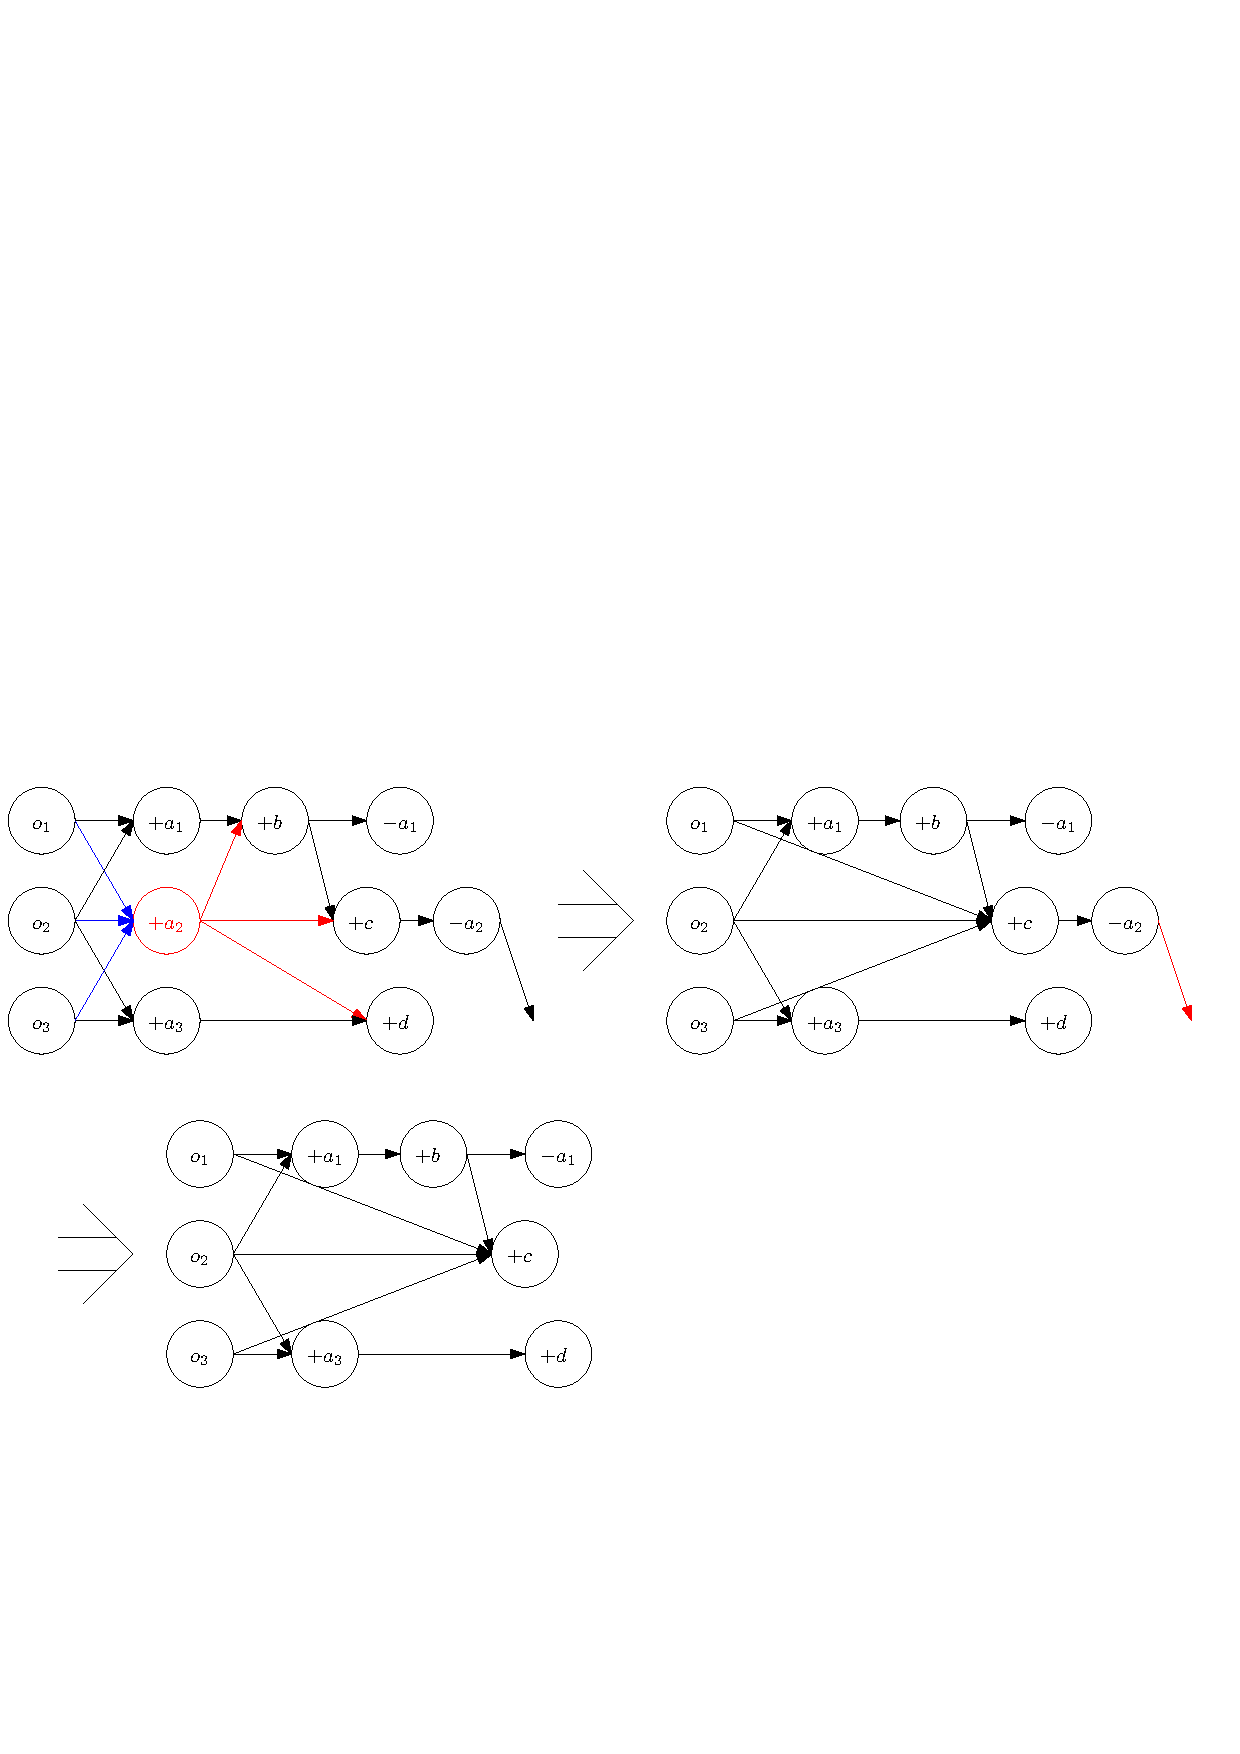
\includegraphics[width=0.8 \textwidth]{figures/PIC-Example-CompactProcess.pdf}
%\vspace{-10pt}
  \caption{The process of penetrating operations $+a_2$ and $-a_2$}
  \label{fig:the process of penetrate operations}
\end{figure}

\figurename~\ref{fig:the process of penetrate operations} shows an example of first penetrate $+a_2$ (from \figurename~\ref{fig:the process of penetrate operations} (a) to \figurename~\ref{fig:the process of penetrate operations} (b)) and then penetrate $-a_2$(from \figurename~\ref{fig:the process of penetrate operations} (b) to \figurename~\ref{fig:the process of penetrate operations} (c)). This is an practical example for the case of OR-set algorithm \cite{Shapiro:2011,Bieniusa:2012}. In \figurename~\ref{fig:the process of penetrate operations} (a), $o_{ip}(+a_2) = o_2$, $o_{is}(+a_2) = +c$, and we explicitly draw $O_{to}(+a_2)$ and $O_{to}(+a_2)$ with blue and red color, respectively. In \figurename~\ref{fig:the process of penetrate operations} (b), $o_{ip}(-a_2) = +c$, $o_{is}(-a_2) = \epsilon$, $O_{to}(-a_2) = \emptyset$ and we explicitly draw $O_{to}(-a_2)$ with red color.

It is not hard to see that, the visibility among operations not penetrated remains the same after penetrating. Therefore, penetrating using different order lead to same consequence.

Given a plus-minus specification $Spec$, its compacted reference implementation is given as an tuple $CRImp(Spec) = (Q,\Sigma,vis,q_0,li,\rightarrow_c,livReq)$. $CRImp(Spec)$ can be obtained from $RImp(Spec) = (Q,\Sigma,vis,q_0,li,\rightarrow,livReq)$ by only changing the transition rules as follows:  $\rightarrow_c = \{ q_1 {\xrightarrow{\alpha}}_c q_2 \vert q_1 {\xrightarrow{\alpha}} q_3 \wedge q_2 = pent(q_3) \}$.

Let $poSet(\llbracket CRImp(Spec) \rrbracket)$ (resp., $poSet(\llbracket RImp(Spec) \rrbracket)$) be the sets of sequences obtained by using poset upon sequences in $\llbracket CRImp(Spec) \rrbracket$ (resp., $\llbracket RImp(Spec) \rrbracket$). The following lemma stats that $poSet(\llbracket CRImp(Spec) \rrbracket) = poSet(\llbracket RImp(Spec) \rrbracket)$. It is not hard to prove this since when defining transition relation of $CRImp(Spec)$ from that of $CRImp(Spec)$, we replace a state with a equivalent state. Its proof is obvious and omitted.

\begin{lemma}
\label{lemma:CRImpcdSpec and RImpcdSpec contain the same set of trace}
$poSet(\llbracket CRImp(Spec) \rrbracket) = poSet(\llbracket RImp(Spec) \rrbracket)$.
\end{lemma}

Similar as the case of reference implementation, we can add the restriction of causal-delivery into compacted reference implementation.

Given a plus-minus specification $Spec$, its compacted reference implementation with causal delivery is given as an tuple $CRImp_{cd}(Spec) = (Q,\Sigma,vis,q_0,li,\rightarrow_{cd},livReq)$. $CRImp_{cd}(Spec)$ can be obtained from $CRImp(Spec) = (Q,\Sigma,vis,q_0,li,\rightarrow_c,livReq)$ by only changing the transition rules of delivering operations as follows: $\rightarrow_{cd} = \{ q_1 {\xrightarrow{addDel(o,r)}}_{cd} q_2 \vert q_1 {\xrightarrow{addDel(o,r)}}_c q_2 \wedge$ $o$ is minimal w.r.t $<_{hb}$ among operations not visible to replica $r$ in $q_1 \}$.

It is easy to see that $CRImp_{cd}(Spec)$ contains all the traces of $CRImp(Spec)$ that are causal delivery, as stated by the following lemma. Its proof is obvious and omitted.

\begin{lemma}
\label{lemma:CRImpcdSpec contains all the traces of CRImpSpec that are causal delivery}

$\llbracket CRImp(Spec)_{cd} \rrbracket = \{ t \vert t \in \llbracket CRImp(Spec) \rrbracket \wedge t$ satisfies causal delivery $\}$.
\end{lemma}
}
